\section{Direct Air Capture}
Direct air capture is a chemical process during which CO$_2$ is drawn directly from the ambient air using either solid or liquid-based air filtering systems. Compared to the other NETs discussed before, it does not face natural constraints, since the only inputs required are electric energy, heat, and water.
\subsection{Technology characterization}
The primary difference between solid DAC and liquid DAC, besides the sorbent or solvent used, is the scale of deployment. While S-DAC plants consist of a number of modular DAC units that capture CO$_2$ using hierarchically porous materials, and can be deployed on variable scale depending on the location and project goals, L-DAC uses liquid basic hydroxide solutions and is usually deployed on a larger, industrial scale to benefit from economies of scale \parencite{mcqueen_review_2021}.\vspace{2mm}

\begin{wraptable}{r}{7cm}
\vspace*{-\baselineskip}
\begin{tabular}{lrr}
\textbf{Input}                                                      & \textbf{S-DAC} & \textbf{L-DAC} \\ \hline
\begin{tabular}[c]{@{}l@{}}Electricity\\ (kWh tCO$_2^{-1}$)\end{tabular} & 415            & 522.5          \\
\begin{tabular}[c]{@{}l@{}}Heat\\ (kWh tCO$_2^{-1}$)\end{tabular}        & 1291.77        & 2222.4         \\
\begin{tabular}[c]{@{}l@{}}Water\\ (t tCO$_2^{-1}$)\end{tabular}         & 1.8            & 4             
\end{tabular}
  \captionof{table}{DAC input variables (gross)}\label{us-case-table}
  \vspace*{-\baselineskip}
\end{wraptable}

In the present model, the input variables are derived from the literature review conducted by \textcite{eke_comprehensive_2025}. For both, S-DAC and L-DAC, the inputs are electric energy, heat, and water. All inputs are assumed to be drawn from a standard grid, with the carbon intensity assumed to be 400 g kWh$^{-1}$ for electricity, 200 g kWh$^{-1}$ for natural gas, and 500 g t$^{-1}$ for water. In addition, a storage leakage factor of 2\% is assumed. In combination with the carbon emissions from the required input energy (see Table 3.3), this results in leakage rates of 42.53\% before storage ($\alpha_0^4$), and 44.53\% including storage ($\alpha_1^4$) for S-DAC. For L-DAC, due to higher energy consumption, the leakage rates are 65.55\% and 67.55\%, respectively. The high leakage rates show that the energy sources are the primary determinant of DAC efficiency. If fully renewable energy was used, the final LCOCR$^+$ as well as the energy use per net tonne of CO$_2$ removed could be reduced by 50 to 60\%.

\subsection{Learning rate}
The learning rate refers to a phenomenon first described by Theodore Wright in relation to the construction of aircraft \parencite{wright_factors_1936}. He observed that with each doubling of the cumulative amount of aircraft manufactured, the production cost dropped by about 20\%. A similar effect was observed more recently in the production of solar PV modules, for which a learning rate of about 33\% was estimated \parencite{irena_renewable_2025}. Similar effects of lesser magnitude were observed for other renewable energy sources, such as wind turbines \parencite{shrestha_learning_2022}.\vspace{2mm}

In mathematical terms, the learning effect can be expressed as the cost reduction dependent on the quantity increase:
\begin{equation}C(Q) = C_0\left(\frac{Q}{Q_0}\right)^{log_2(1-\lambda)}\end{equation}
where $C(Q)$ is the cost at quantity Q, $C_0$ is the initial cost at quantity $Q_0$, and $\lambda$ is the learning rate, i.e. the relative cost reduction assumed for each doubling of cumulative quantity. Figure 3.11 shows the CapEx development of solid DAC, starting from 1.800 USD for the first megatonne. The literature generally expects learning rates between 5 and 15\% for the S-DAC CapEx \parencite{wei_unlocking_2025, al-juaied_prospects_2023, fasihi_techno-economic_2019}. The learning rates for liquid DAC are expected to be significantly lower due to the nature of L-DAC plants, which are typically large-scale industrial plants, as opposed to the modular S-DAC plants \parencite{mcqueen_review_2021}.\vspace{2mm}

\begin{figure}[ht]
  \begin{center}
    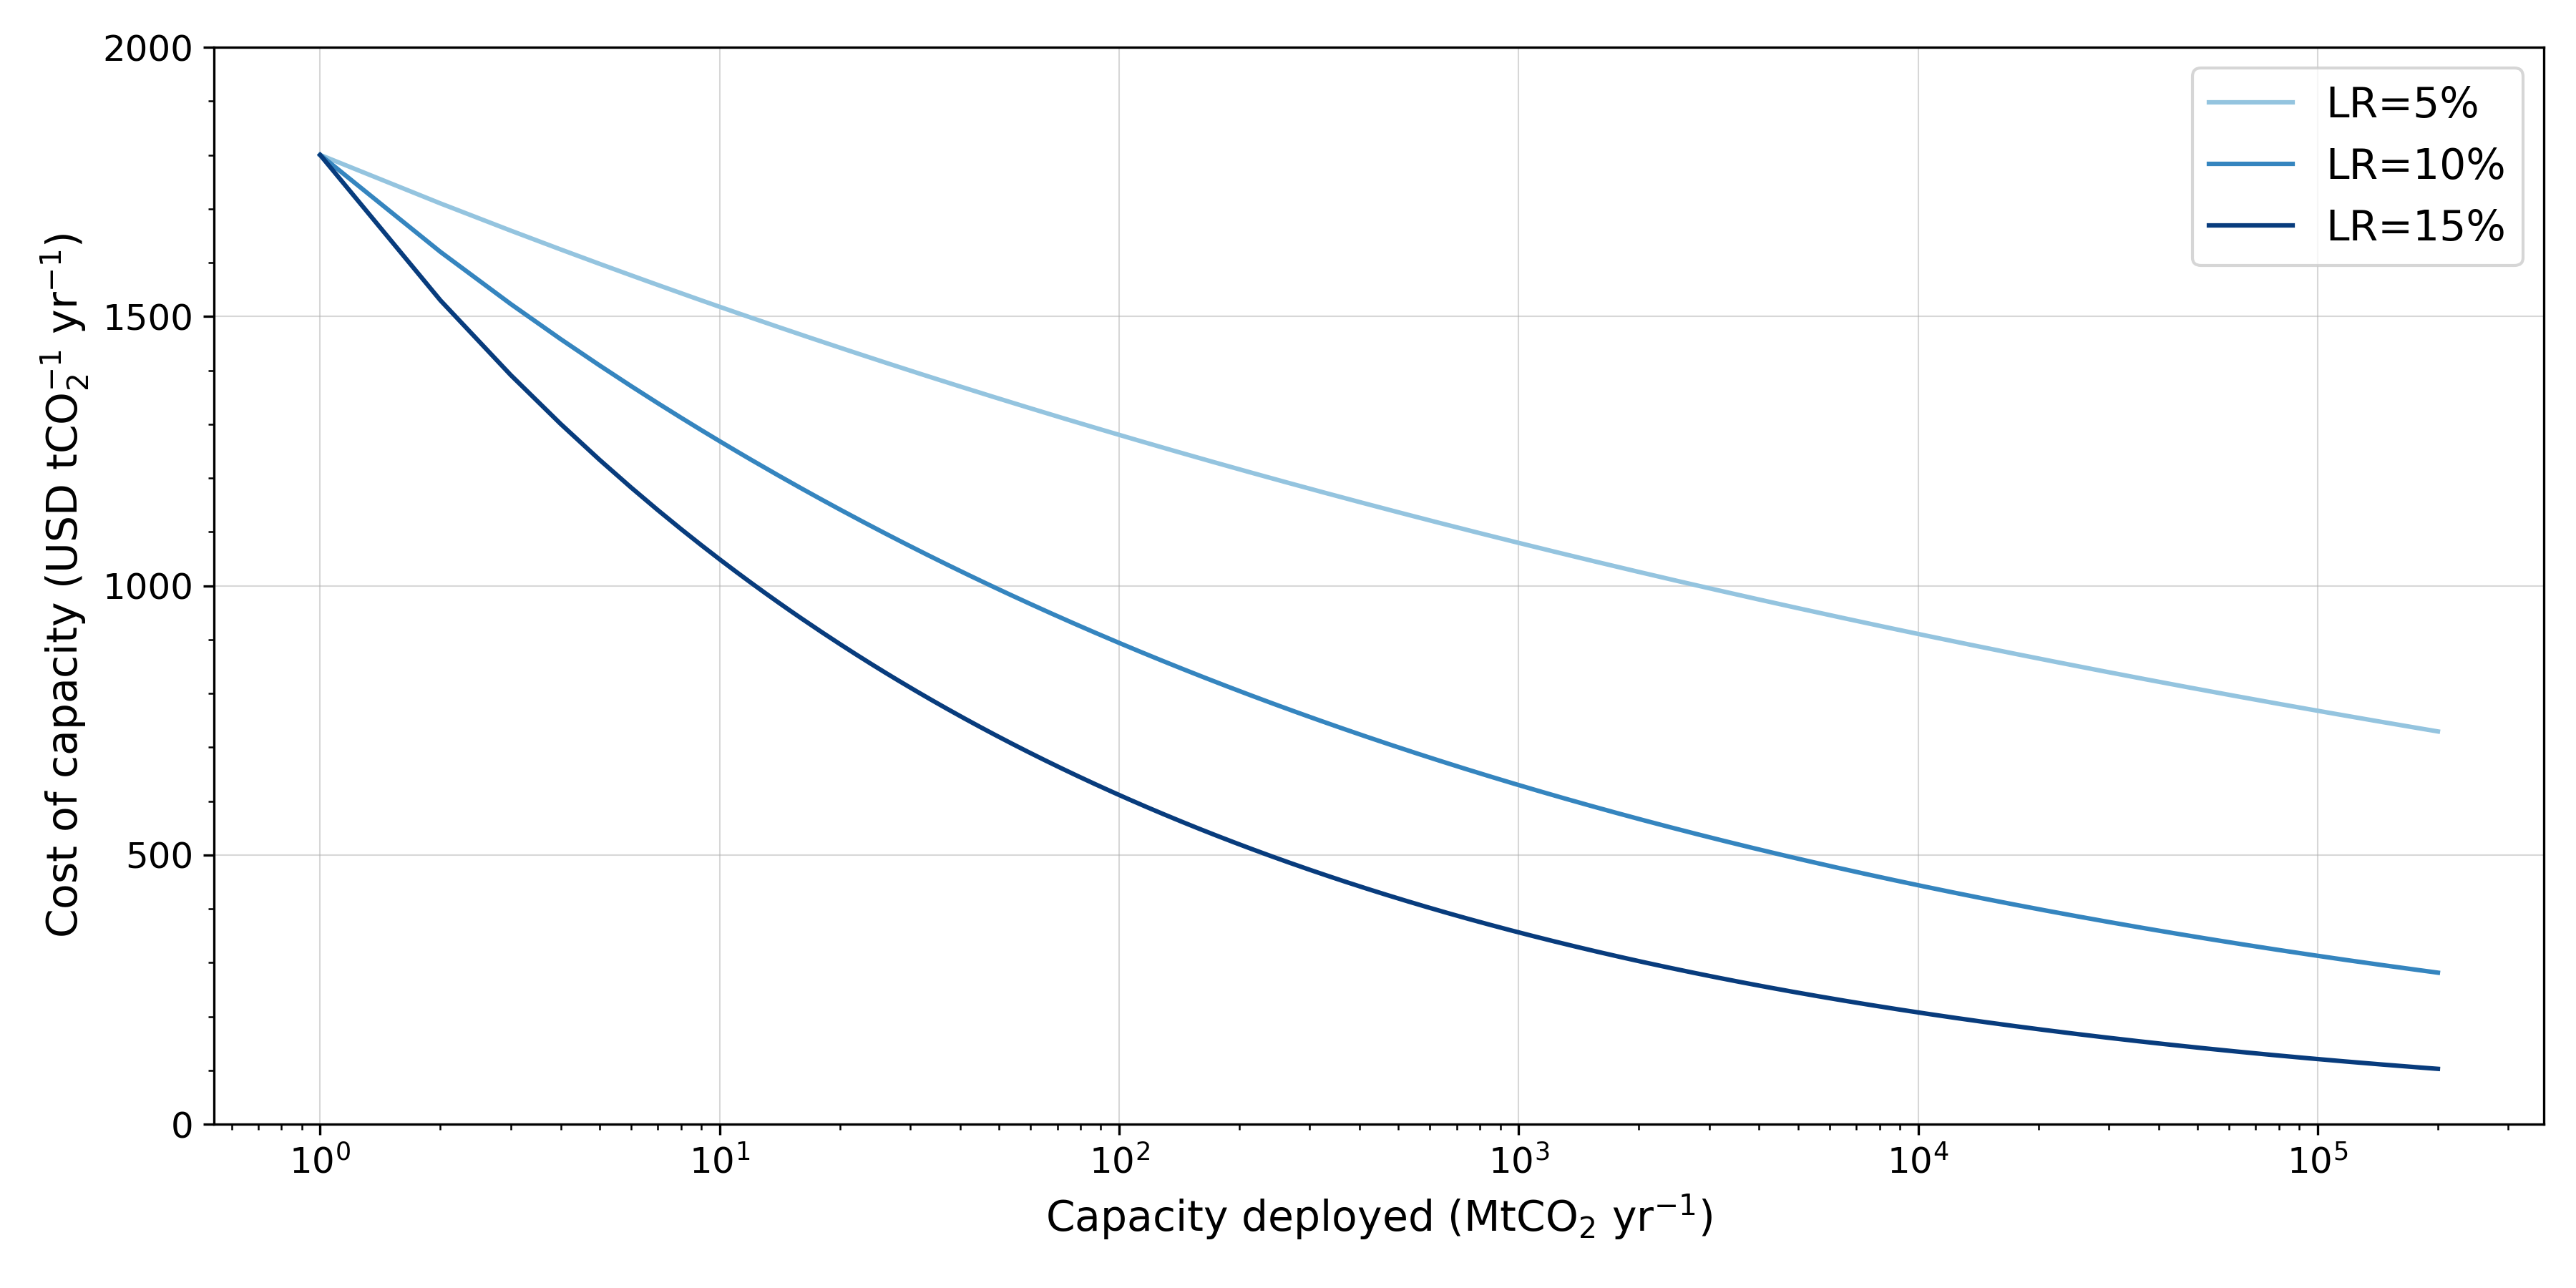
\includegraphics[width=1\linewidth]{figures/dac_learning.png}
    \caption{Exemplary solid DAC CapEx learning curve}
    \label{fig:dac_learning_curve_sdac}
  \end{center}
  \vspace*{-\baselineskip}
\end{figure}

\subsection{Cost model}
The cost of DAC is modeled based on the same assumed 20 year unit lifetime as BECCS, with the costs declining on a learning curve as described above.\vspace{2mm}

The initial cost per tonne of capacity is estimated to be 1.800 USD for S-DAC and 1.000 USD for L-DAC \parencite{stolten_neue_2022}. Further cost components are the cost for electricity and heat from natural gas at 44 USD MWh$^{-1}$ and 30 USD MWh$^{-1}$, respectively, as well as the cost of water at 2 USD t$^{-1}$. Maintenance material costs are assumed to be 2.2\% of CapEx annually, with another 40\% of this material cost added as maintenance labor cost. The transport and storage cost is set at a fixed amount of 11.22 USD tCO$_2^{-1}$, based on the estimate by \textcite{smith_cost_2021} for a 100 mile transport distance (which is lower than that for BECCS due to the location flexibility of DAC) and medium-scale storage project. \vspace{2mm}

Using learning rates of 10\% (S-DAC) and 6\% (L-DAC) yield an initial LCOCR$^+$ of 527.23 USD for S-DAC and 728.51 USD for L-DAC, which decrease to 373.04 (630.46) at 100 MtCO$_2$ yr$^{-1}$, and 328.13 (594.63) at 1 GtCO$_2$ yr$^{-1}$. These results show that DAC is a comparatively expensive approach. While the costs will likely decrease due to experience and learning effects, the exact magnitude of these effects remains somewhat speculative. As Figure 3.11 shows, a lower realized learning rate would quickly make both types of DAC uneconomical. This risk seems especially pronounced for L-DAC, which requires large industrial plants as opposed to the modular nature of S-DAC. Technologies of this type, such as nuclear power stations, have historically seen very low or even negative learning rates and remained expensive \parencite{mcqueen_review_2021}.

\subsection{Constraints}
As discussed before, direct air capture does not face natural constraints of land availability, since the geographic footprint of DAC plants is relatively small relative to their carbon capture capacity, especially compared to A/R. However, DAC consumes significant amounts of energy, including electric energy. At present, the largest direct air capture plant in operation, the \textit{Mammoth} S-DAC plant in Iceland, consumes about 5,000 kWh of electric energy per tonne of CO$_2$ captured \parencite{alexandersson_climeworks_2025}, which is more than double the amount considered in this model. While this plant was not constructed for energy efficiency, and the energy efficiency of DAC is expected to increase, its energy use remains a significant issue. For comparison, at the gross energy intensity described in Table 3.4, compensating 10\% of Germany's 2024 CO$_2$ emissions of 649 Mt \parencite{uba_indicator_2025} would  require 27 TWh of electric energy and 84 TWh of heat if S-DAC was used. This would amount to about 5\% of Germany's electricity generation an 10\% of its natural gas use in the same year \parencite{bundesnetzagentur_bundesnetzagentur_2025, bundesnetzagentur_bundesnetzagentur_2025-1}. Considering the energy consumption described is a gross number and does not consider leakage, the net results might be nearly twice as high at the current grid carbon intensity.\vspace{2mm}

One option to reduce the (net) energy consumption is to use renewable energies, such as solar PV and biogas, to power direct air capture. This would reduce the carbon emissions of the energy used, which in turn would reduce the leakage rate, and therefore the energy required per net tonne of CO$_2$ captured. Still, even at a 0\% leakage rate, the energy consumption of large-scale DAC would make up a significant share of the global energy supply. As discussed in section 2.6, in combination with the greatly increasing energy demand from artificial intelligence, the large-scale deployment of DAC will therefore require the deployment of vast additional, preferably low-carbon, energy sources.